%ब 

\section{Update} \label{s:results-update}
In all the solutions, the \texttt{update} operation triggers a referential
integrity validation whenever any entity of \texttt{Student}, \texttt{Course}
and \texttt{Enrolment} is updated with new values. Figure~\ref{fres:Update}
presents the results of a single update on each entity for all the solutions.
Figure~\ref{fres:Update-responsetime} shows the time taken to compete the
\texttt{update} on each entity in the solutions and
Figure~\ref{fres:Update-throughput} presents the throughput of this operation.

	\begin{figure}[H] 
		\subfigure[Response time for Update operation]
		{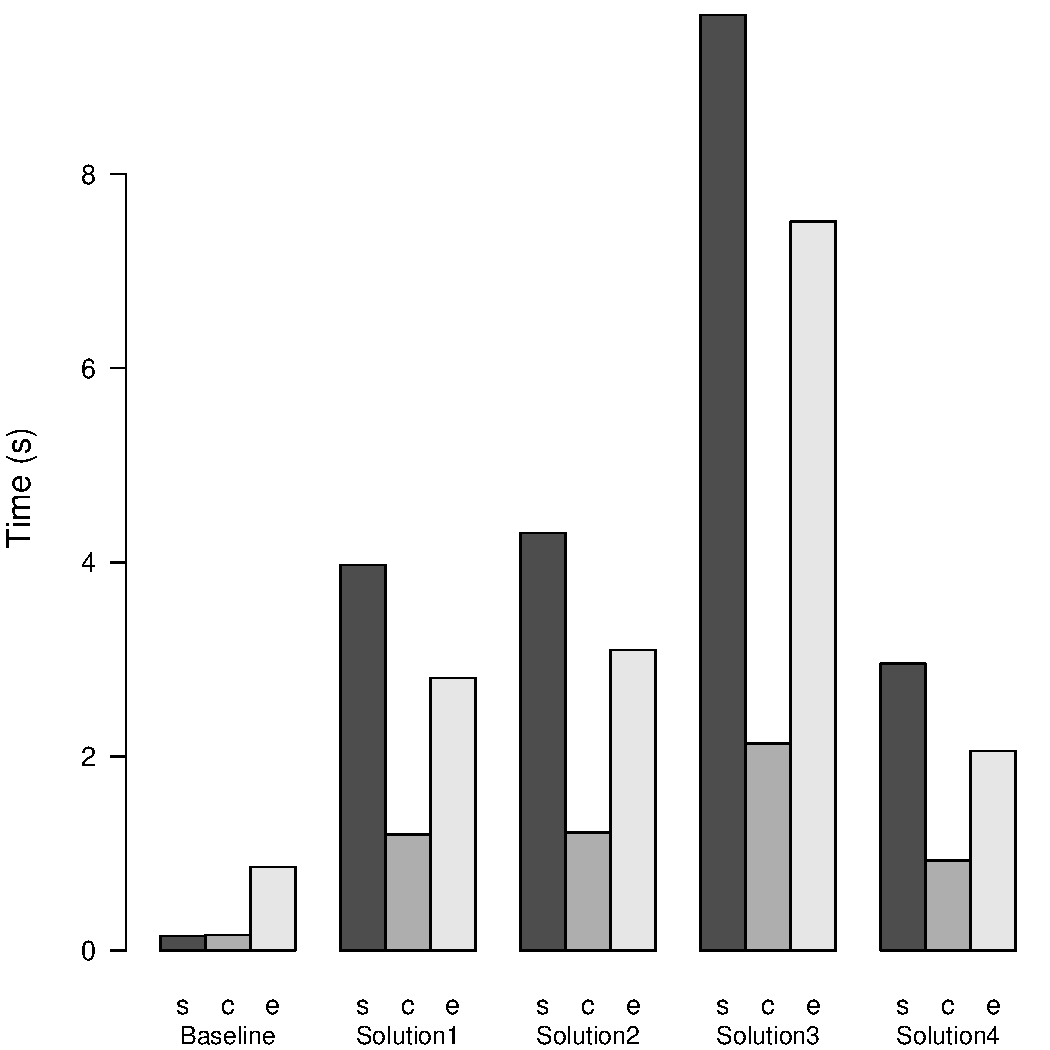
\includegraphics[width=\Width]{figure/result/barplot-update-rt.pdf}\label{fres:Update-responsetime}}
		\subfigure[Throughput for Update operation]
		{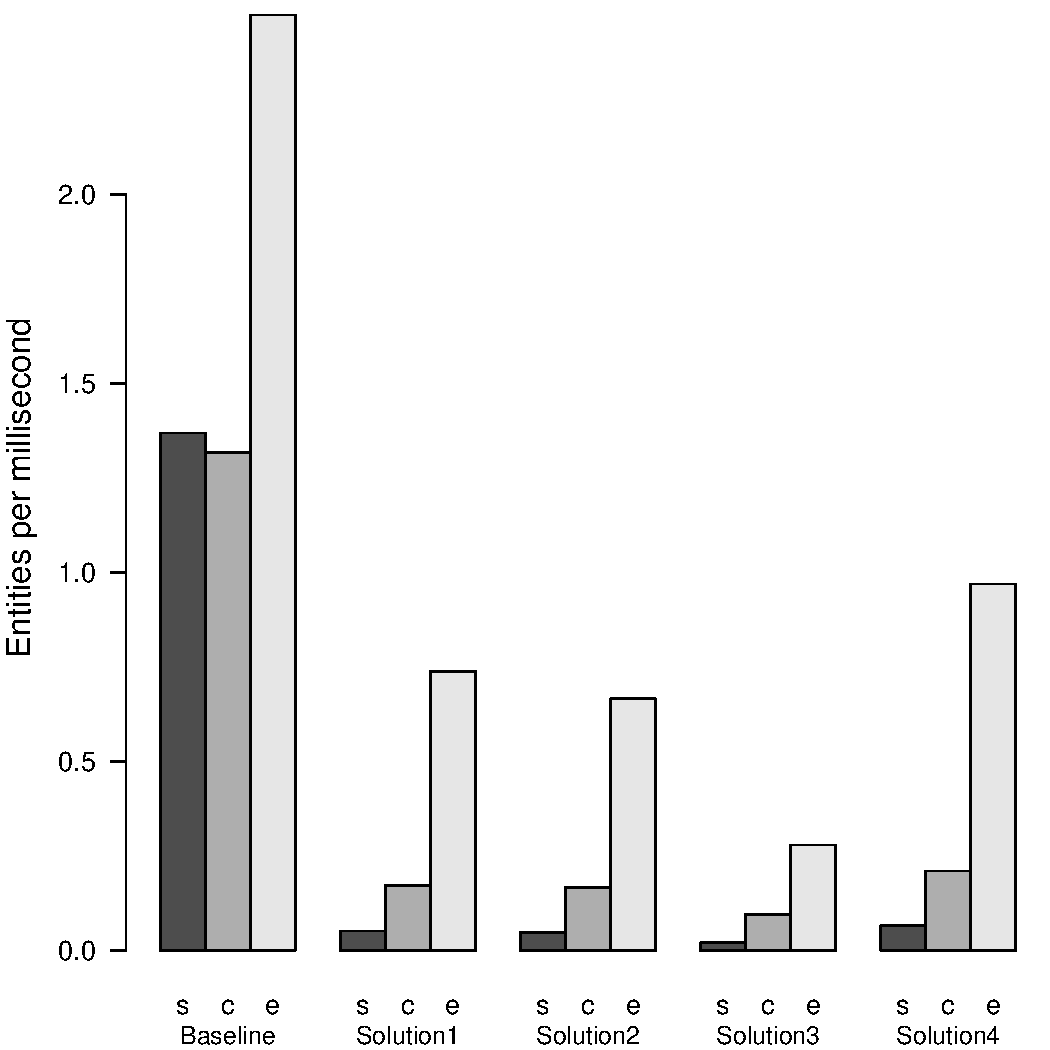
\includegraphics[width=\Width]{figure/result/barplot-update-tp.pdf}\label{fres:Update-throughput}}
		\caption{Performance of Solutions in Update}\label{fres:Update}
	\end{figure}
 
It can be seen from the results that the
\texttt{update} on \texttt{Enrolment} is the fastest in all the solutions, when
compared to \texttt{update} on other entities. On the contrary, \texttt{update}
on a \texttt{Student} entity takes the most time in all the solutions.
\texttt{update} on a \texttt{Course} entity always takes more time than
\texttt{update} on \texttt{Enrolment} but is faster than updating
\texttt{Student} entities.

These differences in the performance of an \texttt{update} on the three entities
is because of the referential integrity rules that are applied during
validation.
% which causes \texttt{update} on parent entities take more time than updating
% child entities.
Updating \texttt{Enrolment} is fastest since it involves only identifying
relevant \ac{FK} constraints in the list of constraints and then accessing the
parent column families \texttt{Student} and \texttt{Course} to verify if the new
foreign key values exist or not. After this, the new values are written to only
the \texttt{Enrolment} column family. 

However, updating a \texttt{Student} entity takes the most time since it is
a cascaded operation. After accessing its relevant \ac{FK} constraints, its
child dependencies are retrieved from \texttt{Enrolment} and updated with the new
value for the \texttt{StudentId}. This means that an \texttt{update}
accesses the metadata as well as the child column family and causes writes not
only in \texttt{Student} but also in the child column family \texttt{Enrolment}.
\texttt{update} on \texttt{Course} entities take lesser time than this because
its not a cascaded operation as the \texttt{DeleteRule} for \texttt{Course}
entities is \texttt{NoDelete}. Thus, exceptions are raised each time an
\texttt{update} is performed on \texttt{Course} entities, which means that the
response time includes measuring the time for validation as well as raising
exceptions. But this is slower than \texttt{update} on \texttt{Enrolment}
because it involves accessing the \texttt{Enrolment} column family
to identify existing child dependencies. Since these child dependencies exist
when the experiments are run, the exceptions are raised each time.

% The time involved for an \texttt{update} on a \texttt{Course} entity is  more as
% seen in Figures~\ref{fres:Update} and~\ref{fres:update-course}. In this
% operation the relevant \texttt{FK} constraints and child dependencies of the
% \texttt{Course} entity are identified and its  relevant \texttt{DeleteRule}
% is also determined.
% Since the \texttt{DeleteRule} for \texttt{Course} entities is \texttt{NoDelete}
% an exception is raised. Moreover, \texttt{Enrolment} column family is accessed
% to identify existing child dependencies. These additional operations and the
% exceptions raised make \texttt{update} on \texttt{Course} consume more time to
% complete.
% 
% The results in Figures~\ref{fres:Update} and~\ref{fres:update-user} show that
% updating a \texttt{Student} entity takes the most time in all the solutions.
% The relevant \ac{FK} constraints are accessed for this entity and
% its child dependencies are identified from \texttt{Enrolment}, which is similar
% to \texttt{update} on \texttt{course} entities. However, update on a
% \texttt{Student} entity is cascaded and involves updating all the child
% dependencies in \texttt{Enrolment} column family. This means that an
% \texttt{update} causes writes not only in \texttt{Student} but also in the child
% column family \texttt{Enrolment}. 
Note that \texttt{update} on \texttt{Student} entities causes values in
two column families to be updated, while in \texttt{Enrolment} values are
updated in only one column family and in \texttt{Course} no values are updated. 


Further details of the performance of each solution when an
\texttt{update} operation is executed on each entity is presented in 
Figures~\ref{fres:update-user},~\ref{fres:update-course}
and~\ref{fres:update-enrolment}.
% These figures show the response time to
% complete one \texttt{update} on all the three entities in every solution and
% the throughput of the operation.
Figure~\ref{fres:update-user} presents the results for an \texttt{update} on a
single \texttt{Student} entity in all the solutions and
Figures~\ref{fres:update-course} and~\ref{fres:update-enrolment} show the
performance of an \texttt{update} on a \texttt{Course} and \texttt{Enrolment}
entity in the solutions. These results show that Solution~4 is the fastest
amongst all the solutions, while Solution~3 is the slowest.
Solutions~1 and 2 perform almost similarly although the additional search for
the top row in Solution~2 makes it just slightly slower than Solution~1.
Note that in Solution~3 the \texttt{Metadata} column family is accessed multiple
times in each validation making it the slowest. Multiple accesses are needed in
order to first retrieve the relevant \ac{FK} constraints and then to retrieve
information about the child or parent entities. Although Solution~4 stores
metadata separately like Solution~3, it caches the \texttt{Metadata} column
family and reuses the cache to avoid such multiple accesses to the column
family.

When compared to the baseline, the \texttt{update} operation on all the
entities take considerably more time in all the solutions because of
their different metadata storage designs. The validations and metadata access
for parent entities make Solution~4 20 times slower than the baseline and
Solution~3 almost 60 times slower in cascaded updates, which is the most
time consuming \texttt{update}. 
Solutions~1 and 2 are almost more than 25 times slower than
baseline in such updates. However, updates on child entities make Solution~4
only slightly slower than the baseline while Solution~3 is three times slower.
In such cases, Solution~1 and 2 are almost 1.5 times slower than the baseline.

% Note that in all the solutions the \texttt{update} on . This is because of the different
% referential integrity rules applied on the entities. 
 
\begin{landscape}
		\begin{figure}
		\centering
		\newcommand{\W}{.4\textwidth}
			\subfigure[ Update on Student]
			{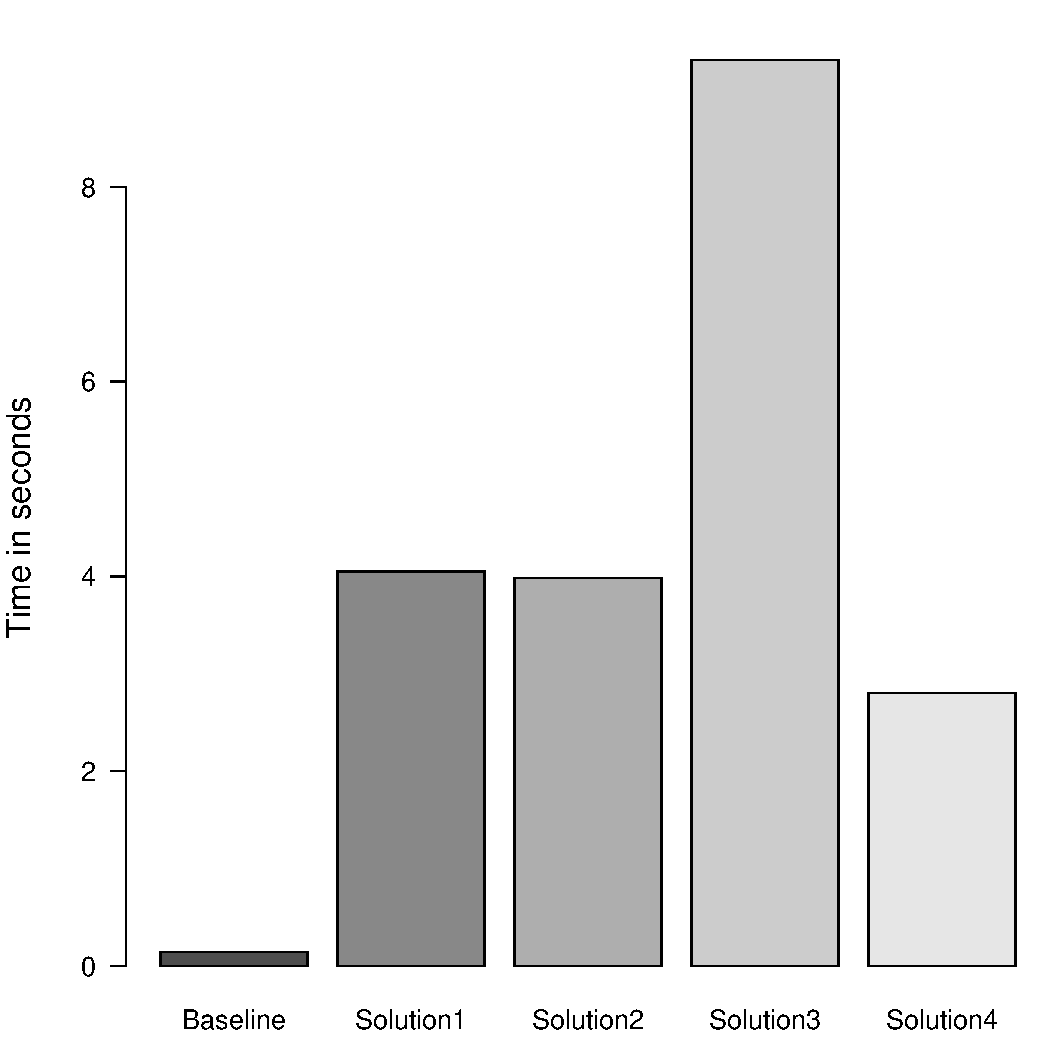
\includegraphics[width=\W]{figure/result/barplot-update_student-rt.pdf}}
			\subfigure[ Update on Course]
			{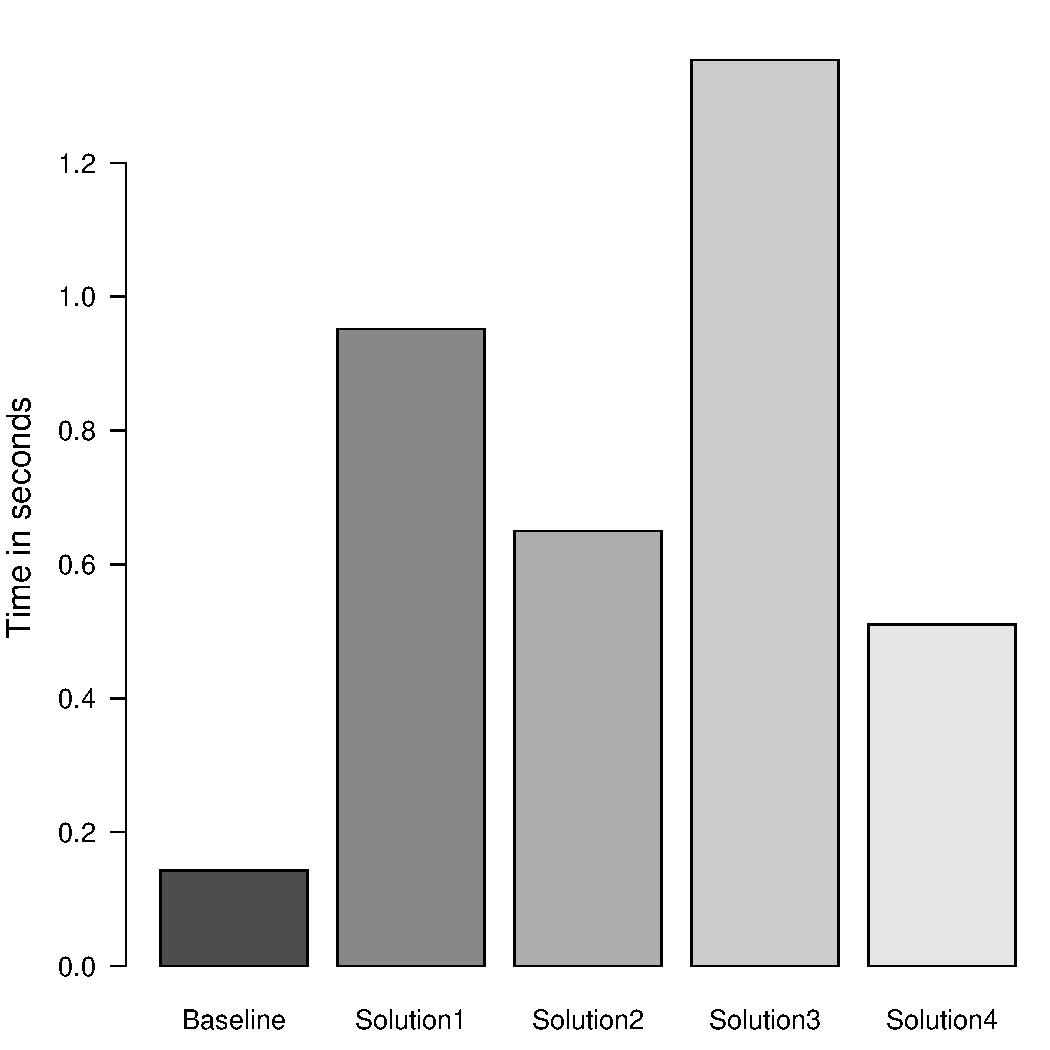
\includegraphics[width=\W]{figure/result/barplot-update_course-rt.pdf}}
			\subfigure[ Update on Enrolment]
			{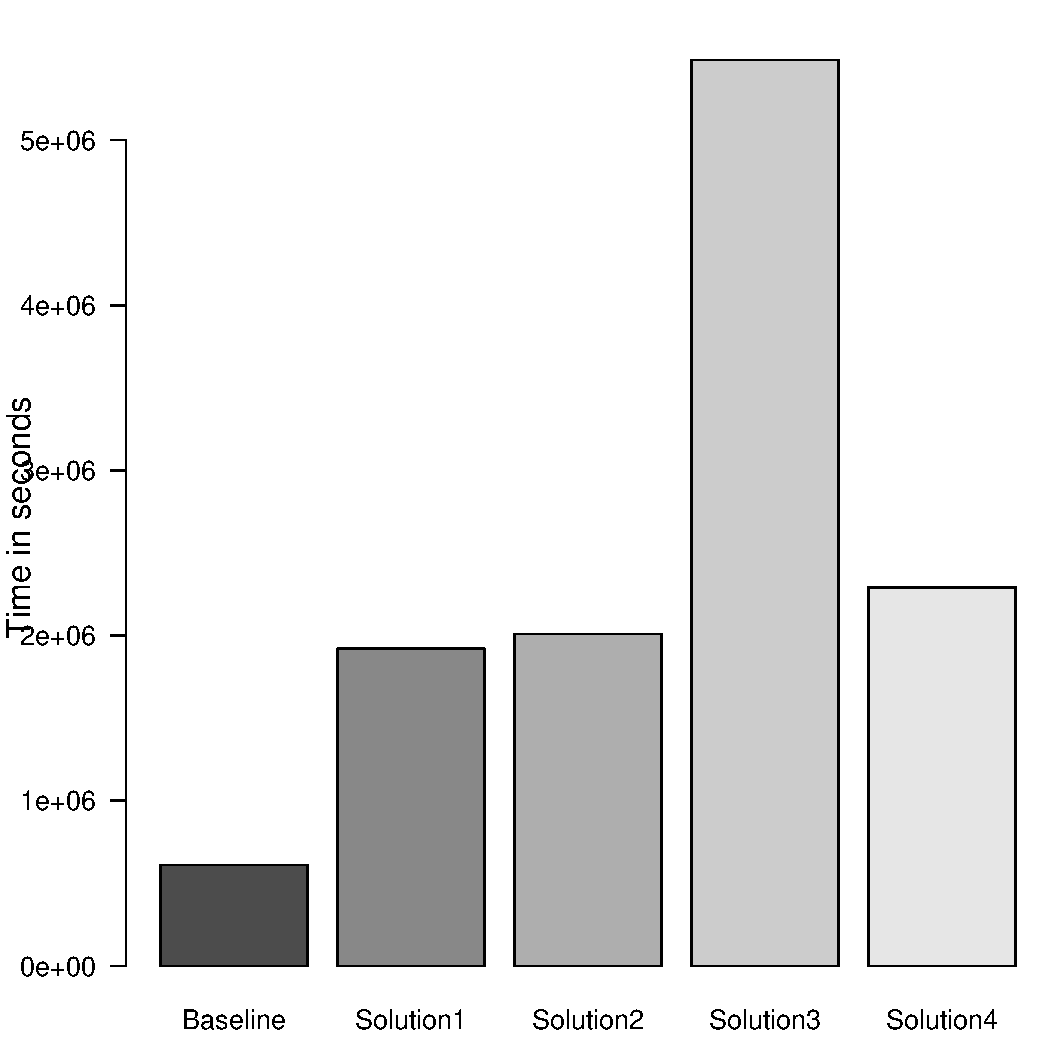
\includegraphics[width=\W]{figure/result/barplot-update_enrolment-rt.pdf}}
			\caption{Response time updating entities}\label{fres:update-response-time}
			
			\subfigure[Update on Student]
			{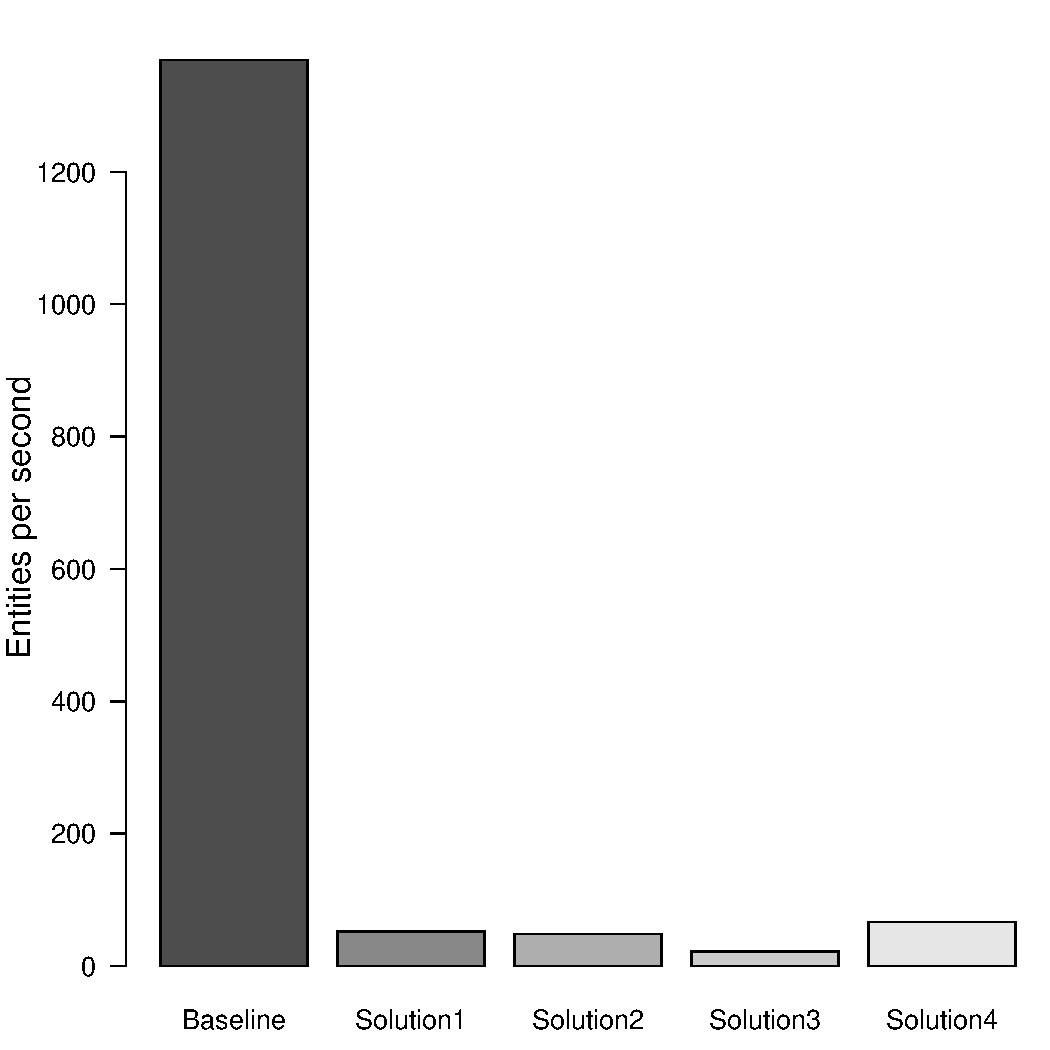
\includegraphics[width=\W]{figure/result/barplot-update_student-tp.pdf}}			
			\subfigure[ Update on Course]
			{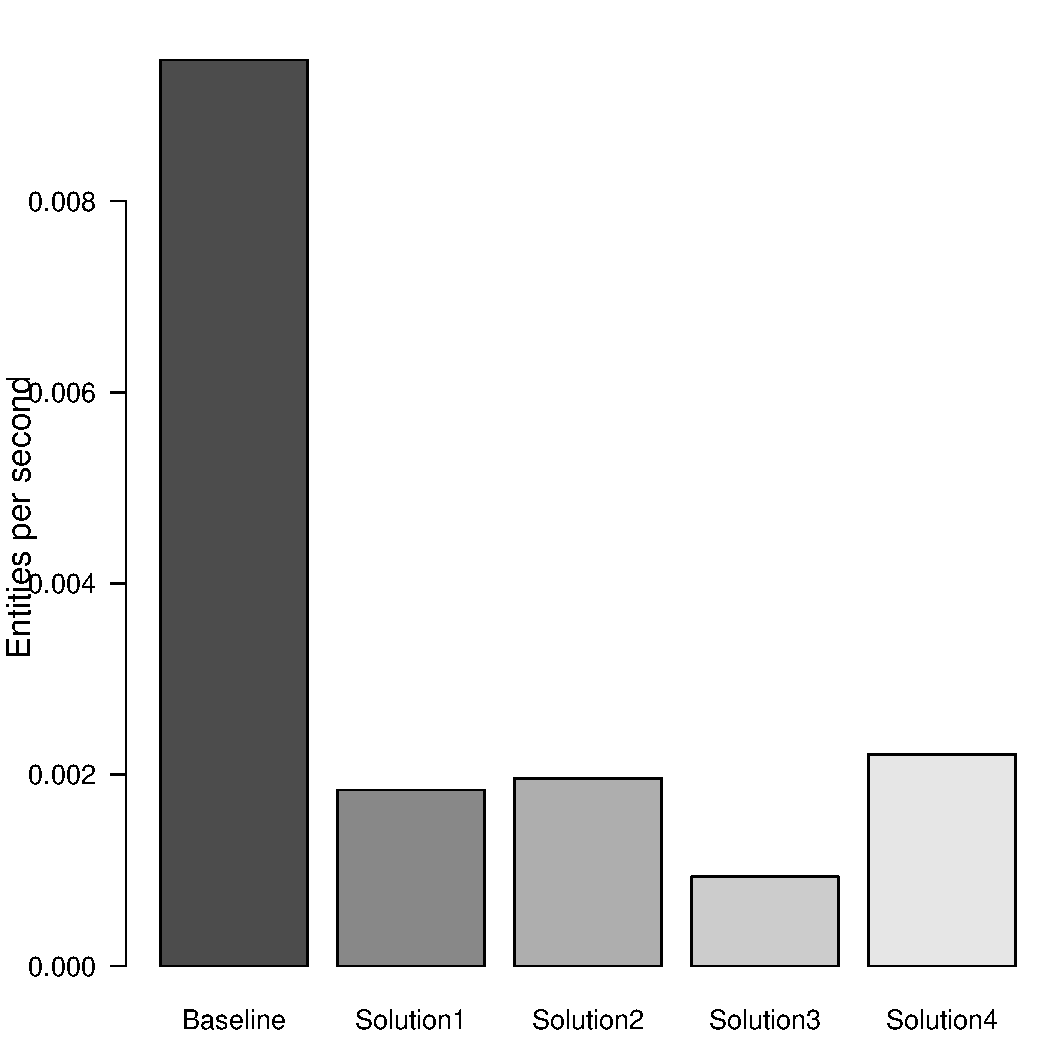
\includegraphics[width=\W]{figure/result/barplot-update_course-tp.pdf}}
			\subfigure[Update on Enrolment]
			{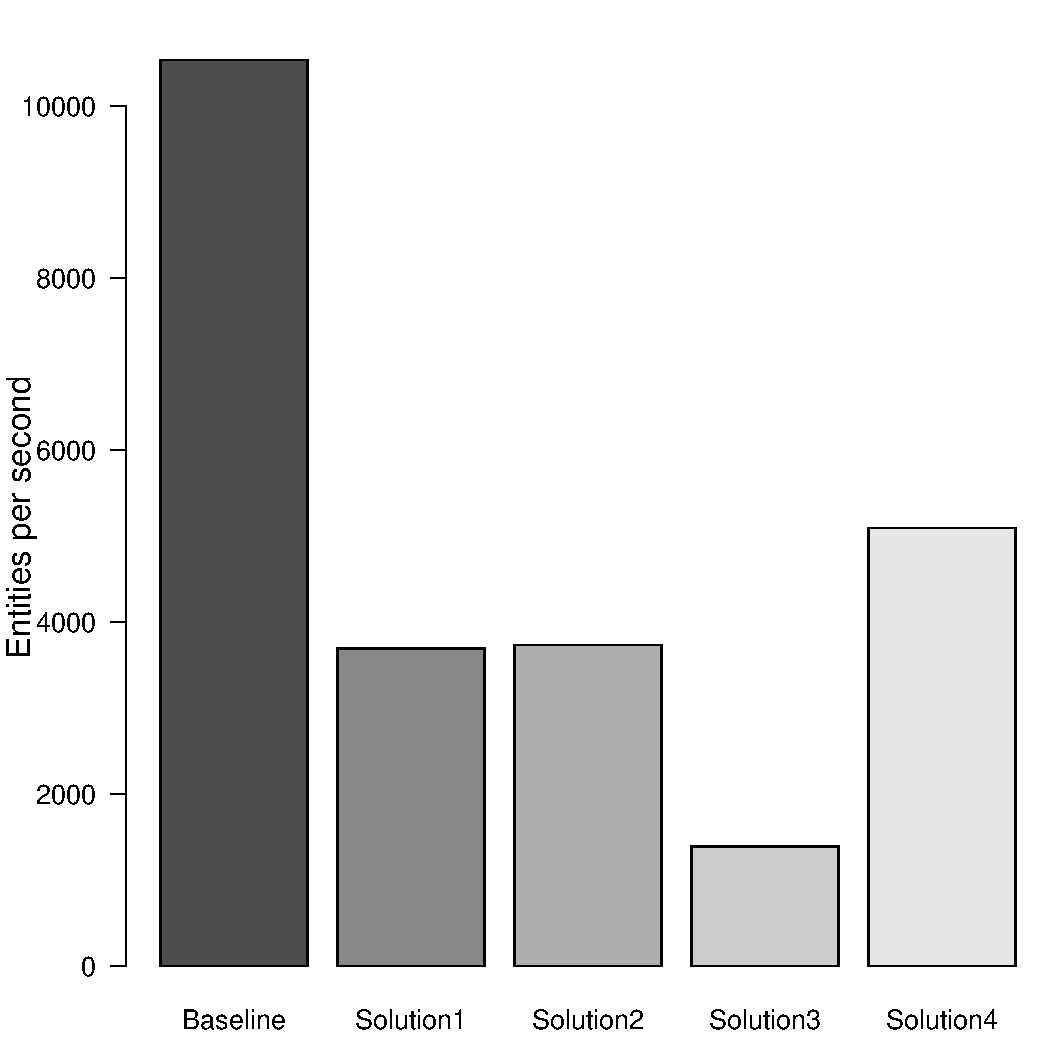
\includegraphics[width=\W]{figure/result/barplot-update_enrolment-tp.pdf}}
			\caption{Throughput updating entities}\label{fres:update-throughput}
		\end{figure}
\end{landscape}